%%%%%%%%%%%%%%%%%%%%%%%%%%%%%%%%%%%%%%%%%
% CV
%
% This CV template is based on:
% https://overleaf.com/latex/templates/cv-developer/rdycxzvvnvcc
% by Omar Roldan
%
% Modified by Yunus Emre Yavuz
%
% License:
% The MIT License (see included LICENSE file)
%
%%%%%%%%%%%%%%%%%%%%%%%%%%%%%%%%%%%%%%%%%

%----------------------------------------------------------------------------------------
%	PACKAGES AND OTHER DOCUMENT CONFIGURATIONS
%----------------------------------------------------------------------------------------

\documentclass[9pt]{developercv} % Default font size, values from 8-12pt are recommended
\usepackage[ngerman, english]{babel}
\setlength{\parindent}{0pt}
\usepackage{multicol}
\usepackage{graphicx}
\usepackage[ddmmyyyy]{datetime}
\renewcommand{\dateseparator}{.}
\setlength{\columnsep}{0mm}
\usepackage{ifthen}
\usepackage{tcolorbox}
\usepackage{parcolumns}
\usepackage{tikz}
% Set the language variable: 0 for German, 1 for English
\newcommand{\lang}{1}

%----------------------------------------------------------------------------------------
\begin{document}

%----------------------------------------------------------------------------------------
%	TITLE AND CONTACT INFORMATION
%----------------------------------------------------------------------------------------

\begin{minipage}[t]{0.5\textwidth} 
	\vspace{-\baselineskip} % Required for vertically aligning minipages
	
	{ \fontsize{16}{20} \textcolor{black}{\textbf{\MakeUppercase{Yunus Emre Yavuz}}}} % First name
	
	\vspace{6pt}
	
	{\Large Student} % Career or current job title
 
    \vspace{18pt}
    
    \icon{Envelope}{11}{\href{mailto:yunus@yuemya.de}{yunus@yuemya.de}}

    \icon{Globe}{11}{\href{www.yuemya.de}{Portfolio: yuemya.de}}
    
    \icon{LinkedinSquare}{11}{\href{https://www.linkedin.com/in/yunuseyvz}{LinkedIn: yunuseyvz}}
    
    \icon{Github}{11}{\href{https://github.com/yunuseyvz}{GitHub: yunuseyvz}}
    
\end{minipage}
\hfill
\begin{minipage}[t]{0.22\textwidth}
\vspace{-\baselineskip}
	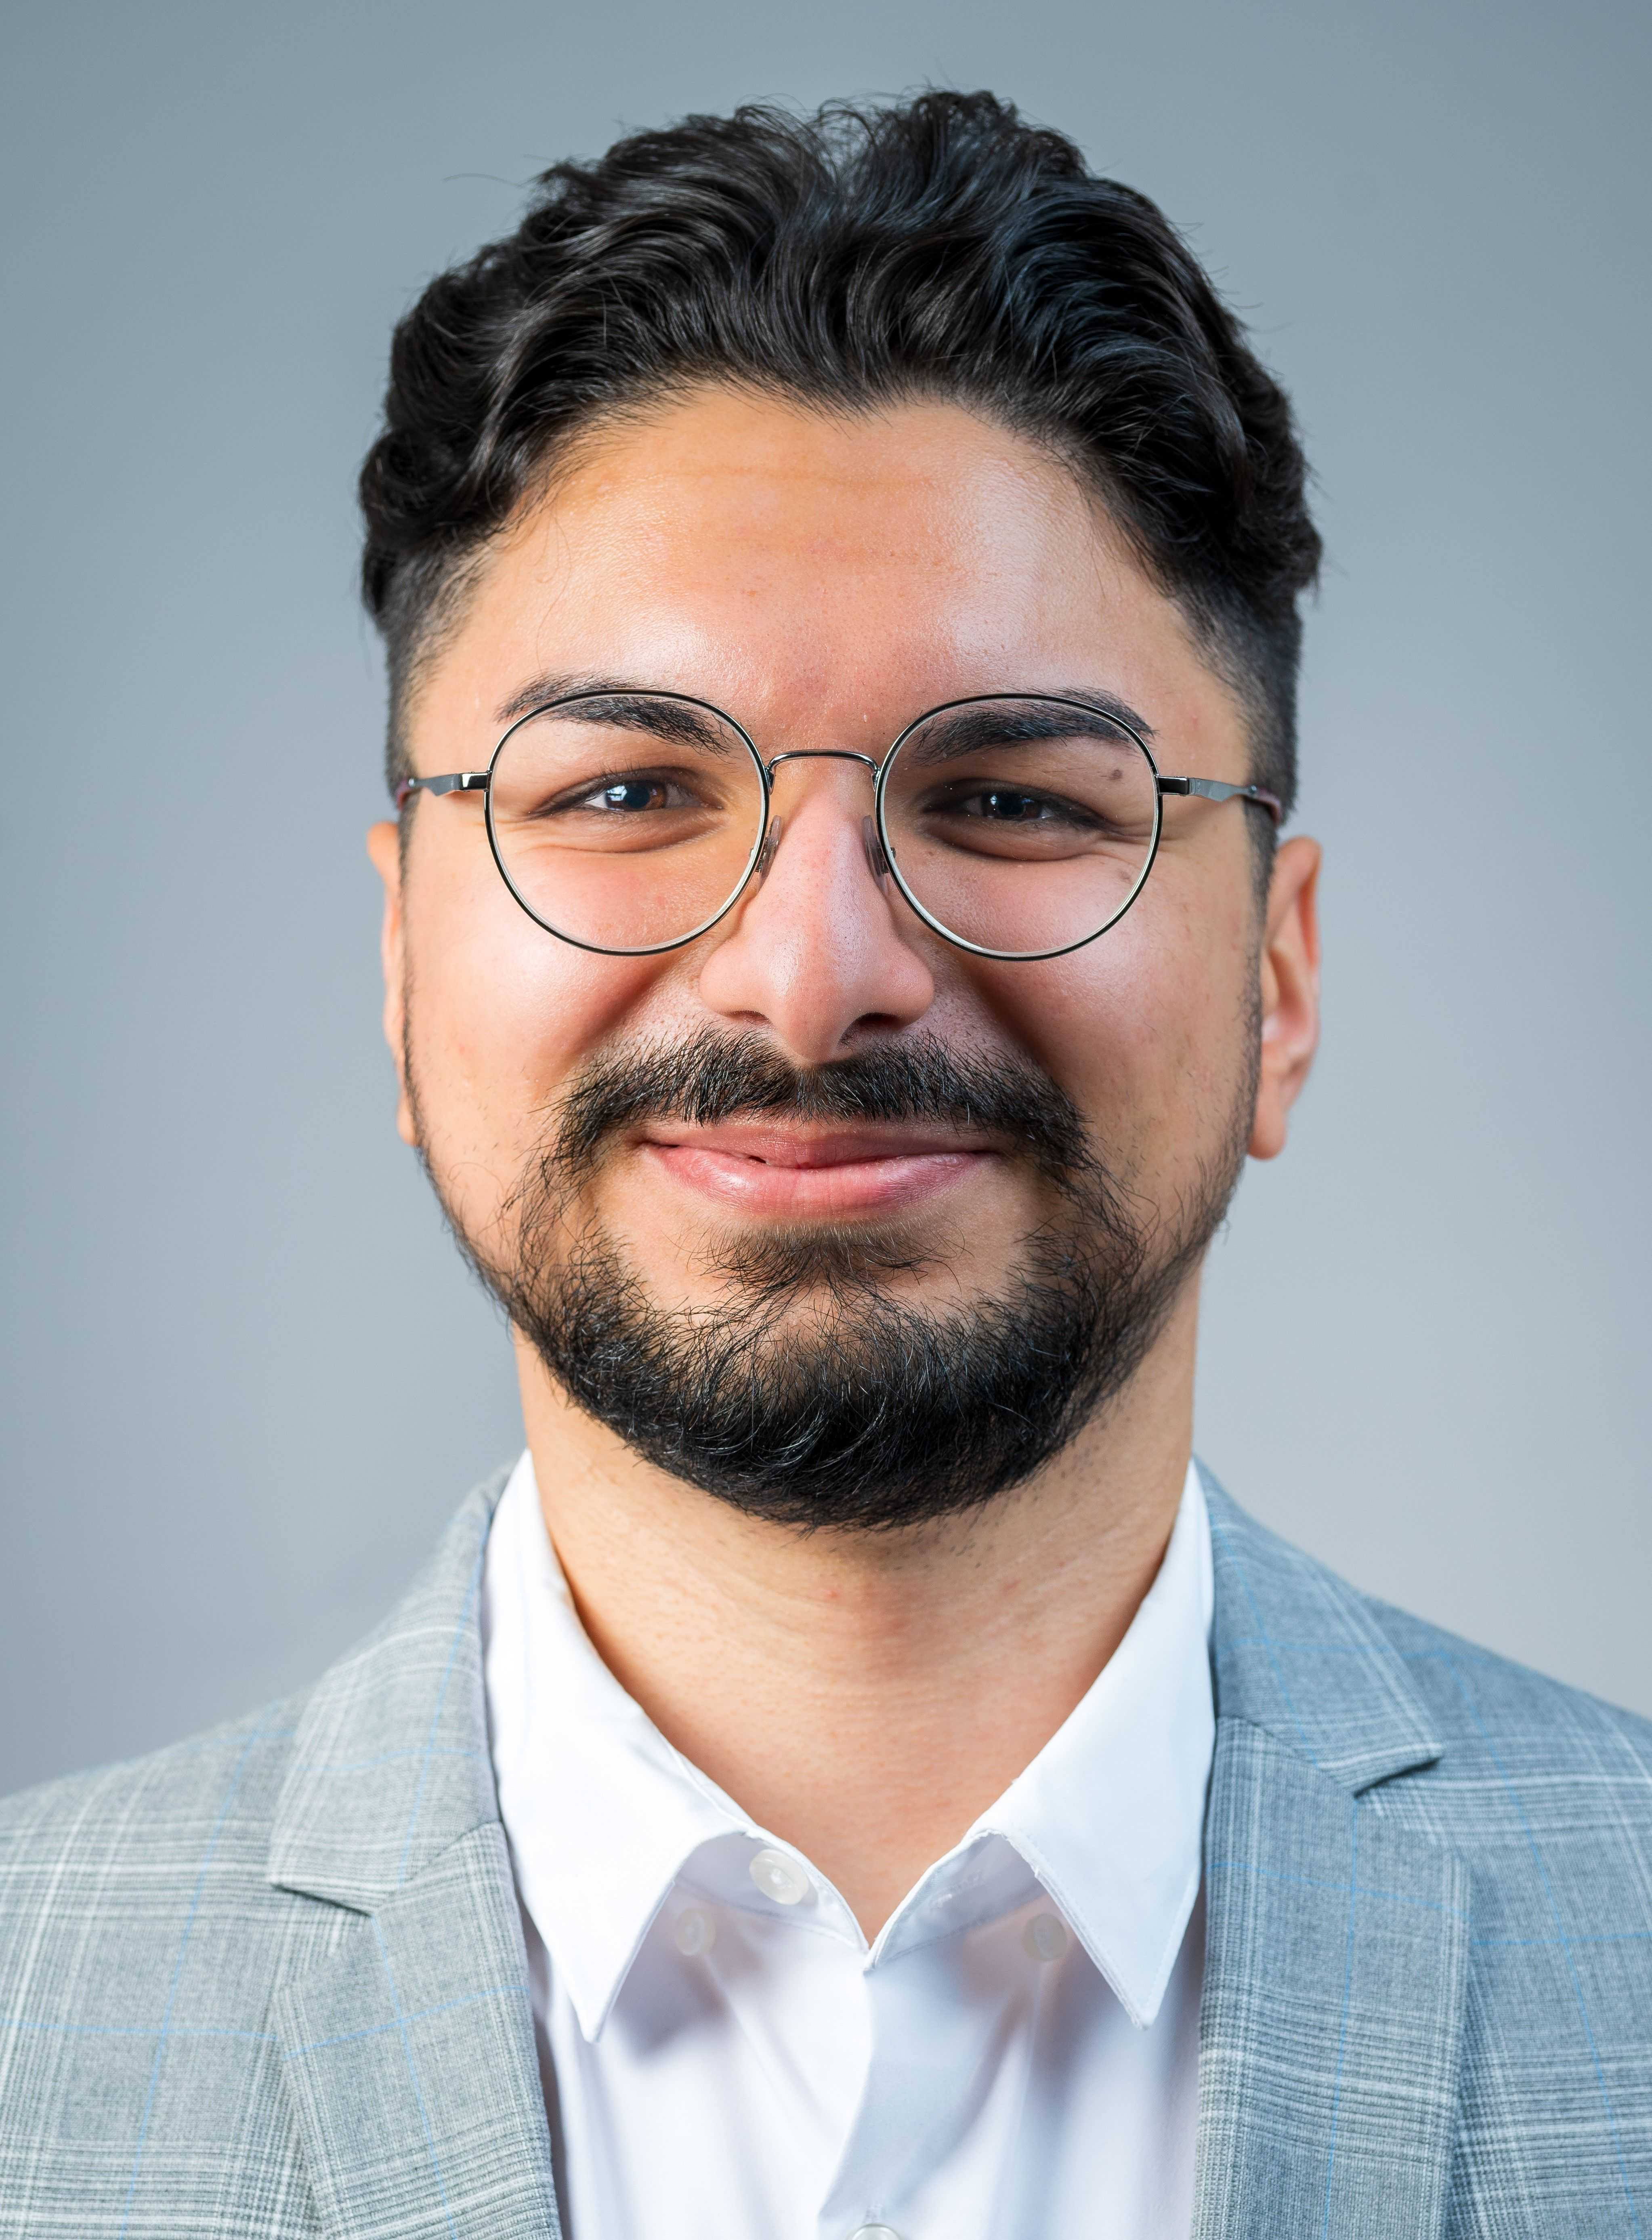
\includegraphics[width=\linewidth]{photo.jpg}
\end{minipage}

%----------------------------------------------------------------------------------------
%	EDUCATION
%----------------------------------------------------------------------------------------
\vspace{10pt}
\ifthenelse{\equal{\lang}{0}}{
    \cvsect{Akademischer Werdegang}
    \begin{entrylist}
        \entry
            {Ab \par 04/2025}
            {LMU München}
            {Human Computer Interaction (M.Sc.)}
            { }
        \entry
            {10/2019 -- \par  03/2025}
            {LMU München}
            {Medieninformatik (B.Sc.), Anwendungsfach Mensch-Maschine-Interaktion}
            {Thema der Abschlussarbeit: Bewertung von Phishing-Warntechniken
            
            Entwicklung und Bewertung verschiedener visueller Phishing-Warnungen in E-Mail-Clients im Rahmen einer Nutzerstudie. Die Studie verwendete Eye-Tracking-Technologie und qualitatives Feedback, um das Benutzerengagement und die Reaktionszeiten zu bewerten und zu verbessern.}
        \entry
            {10/2018 -- \par  09/2019}
            {TU München}
            {Elektro- und Informationstechnik (B.Sc.)}		
            { }
        \entry
            {09/2010 -- \par  06/2018}
            {Adolf-Weber-Gymnasium München}
            {Abitur}
            { }
    \end{entrylist}
}{
    \cvsect{Education}
    \begin{entrylist}
        \entry
            {Starting \par 04/2025}
            {LMU Munich}
            {Human Computer Interaction (M.Sc.)}
            { }
        \entry
            {10/2019 -- \par  03/2025}
            {LMU Munich}
            {Media Informatics (B.Sc.), minor Human Computer Interaction}
            {Thesis Topic: Evaluation of Phishing Warning Techniques
            
            Designed and evaluated different visual phishing warnings in a user study. The study used eye-tracking technology and qualitative feedback to assess and improve the user experience.}
        \entry
            {10/2018 -- \par  09/2019}
            {TU Munich}
            {Electrical Engineering and Information Technology (B.Sc.)}		
            { }
        \entry
            {09/2010 -- \par  06/2018}
            {Adolf-Weber-Gymnasium Munich}
            {Abitur}
            { }
    \end{entrylist}
}

%----------------------------------------------------------------------------------------
%	EXPERIENCE
%----------------------------------------------------------------------------------------
\vspace{-10 pt}
\ifthenelse{\equal{\lang}{0}}{
    \cvsect{Berufserfahrung}
    \begin{entrylist}
        \entry
            {01/2022 -- \par 12/2023}
            {MTU Aero Engines AG}
            {Werkstudent im Bereich IT Quality \& IT Governance}
            {Unterstützung im Software Asset Management durch Organisation, Katalogisierung und Pflege des Softwarebestands des Unternehmens, einschließlich Lizenzen, Abonnements und Nutzungsdaten.}
        \entry
            {05/2019 -- \par 02/2020}
            {Münchener Hypothekenbank eG}
            {Werkstudent im Bereich Immobilienfinanzierung Privatkunden}
            {Überprüfung von Dokumenten, Anforderung fehlender Unterlagen, Pflege von Daten in SAP sowie Korrespondenz mit Kunden, Notaren und Banken.}
    \end{entrylist}
}{
    \cvsect{Experience}
    \begin{entrylist}
        \entry
            {01/2022 -- \par 12/2023}
            {MTU Aero Engines AG}
            {Working Student in IT Quality \& IT Governance}
            {Providing assistance in Software Asset Management by organizing, cataloging, and maintaining the company’s software inventory, including licenses, subscriptions, and usage data.}
        \entry
            {05/2019 -- \par 02/2020}
            {Münchener Hypothekenbank eG}
            {Working Student in Private Client Real Estate Financing}
            {Reviewing documents, requesting missing documentation, maintaining data in SAP, and corresponding with customers, notaries, and banks.}
    \end{entrylist}
}

%----------------------------------------------------------------------------------------
%	SKILLS
%----------------------------------------------------------------------------------------
\tcbset{width=1.5cm,height=.75cm, halign=center,colframe=black!10, colback=black!10, boxsep=-7pt, arc=2mm, nobeforeafter, top=12.5pt}
\vspace{-10 pt}

    \cvsect{Skills}

    \begin{minipage}[t]{0.48\textwidth}
        \textbf{Programming} \\
        
        \tcbox{JS / TS} \hspace{1pt}
        \tcbox{HTML / CSS} \hspace{1pt}
        \tcbox{Java} \hspace{1pt}
        \tcbox{Python} 
        
        \vspace{5pt}
    
        \textbf{Frameworks \& Libraries} \\
        
       \tcbox{React} \hspace{1pt}
        \tcbox{Next.js} \hspace{1pt}
    
        \vspace{5pt}
    \end{minipage}    
    \hfill
    \begin{minipage}[t]{0.48\textwidth}
    
        \textbf{Tools} \\
        
        \tcbox{Git} \hspace{1pt}
        \tcbox{CI/CD} \hspace{1pt}
        \tcbox{WSL} \hspace{1pt}
        \tcbox{REST APIs} \hspace{1pt}
    
        \vspace{5pt}

        \ifthenelse{\equal{\lang}{0}}{
        \textbf{Design \& Forschung} \\
        }{
        \textbf{Design \& Research} \\
        }
        
        \tcbox{Figma} \hspace{1pt}
        \tcbox{User Research} \hspace{1pt}
        \tcbox{Usability Testing} \hspace{1pt}
    \end{minipage}
    
    \ifthenelse{\equal{\lang}{0}}{
        \cvsect{Sprachen}
        
        \tcbox{Deutsch} \hspace{1pt}
        \tcbox{Englisch} \hspace{1pt}
        \tcbox{Türkisch} \hspace{1pt}
        \tcbox{Französisch}
    }{
        \cvsect{Languages}
        
        \tcbox{German} \hspace{1pt}
        \tcbox{English} \hspace{1pt}
        \tcbox{Turkish} \hspace{1pt}
        \tcbox{French}
    }


\end{document}
